\documentclass[../structural_economics_book.tex]{subfiles}
\begin{document}
\ifSubfilesClassLoaded{\setcounter{chapter}{8}}{}
\chapter{Where Preferences Come From}\label{ch:09}
\chaptersubtitle{The Assumption Economics Is Afraid to Touch}
% TODO-VERIFY: epigraph wording not located; check against Furtado, O Mito do
% Desenvolvimento Economico (Rio de Janeiro: Paz e Terra, 1974) and add the page.
% If not found, replace with a verified passage from the same book.
\begin{quote}
\textit{``O mito do desenvolvimento econ\^{o}mico tem exercido, no plano das rela\c{c}\~{o}es internacionais, uma fun\c{c}\~{a}o similar \`{a}quela desempenhada, no plano das rela\c{c}\~{o}es de classe, pelos mitos criados pela ideologia da classe dominante.''}\\[0.3em]
\textnormal{[``The myth of economic development has exercised, in the plane of international relations, a function similar to that performed, in the plane of class relations, by the myths created by the ideology of the dominant class.'']}\\
\hfill --- Celso Furtado, \textit{O Mito do Desenvolvimento Econ\^{o}mico} (1974)
\end{quote}
\nocite{furtado1974mito}

\vspace{1em}

Part~II derived the allocation from the weight matrix: given $(W, \boldsymbol{\omega}, \boldsymbol{\theta})$, the bargaining equilibrium produces $\x^*$. The weights $\boldsymbol{\pi}(W)$ and endowments $\boldsymbol{\omega}$ were computed; the preference vector $\boldsymbol{\theta}$ was assumed.

This chapter removes the last exogenous object. It asks: where does $\boldsymbol{\theta}$ come from?

The answer proposed here is $W^I$: preference parameters are modelled as the output of a formation process driven by the outcomes an agent observes, and which outcomes she observes is set by the information network. A discount factor, an aspiration level, or a labor-supply norm then becomes a function of the $W^I$-weighted returns of an agent's reference group rather than a draw from a fixed distribution.

This is Part~III's working hypothesis: \textbf{preference parameters that the benchmark model treats as primitives can be modelled as the output of a formation process mediated by $W^I$.} Section~\ref{ch09:sec:beliefs} asks how much of the evidence is about preferences rather than beliefs. Chapter~10 will write the formal model. Chapter~11 will measure the formation effect empirically. Chapter~12 will ask what happens to welfare analysis when the welfare function is endogenous. This chapter lays the conceptual and empirical foundation.


%% =====================================================================
\section{The \textit{De Gustibus} Assumption}
\label{ch09:sec:degustibus}
%% =====================================================================

\subsection{What Economists Assume}

In 1977, George Stigler and Gary Becker published ``De Gustibus Non Est Disputandum'' in the \textit{American Economic Review} \citep{stigler1977gustibus}. Their argument: economists should not try to explain tastes. Tastes are stable, exogenous, and uniform across agents (or at least randomly distributed). All observable differences in behavior can be explained by differences in prices and constraints, not differences in preferences.

This is assumption A6 from Chapter~4: $\boldsymbol{\theta}$ is fixed. It is the deepest assumption in the standard model --- the one that makes all other analysis possible. If preferences are exogenous, the economist's job is to study how constraints (prices, endowments, institutions) map into outcomes. If preferences are endogenous, everything changes: the constraints shape the preferences that evaluate the outcomes that the constraints produce.

\begin{definition}[The Preference Vector]\label{ch09:def:theta}
The \textbf{preference vector} $\boldsymbol{\theta} = (\theta_1, \ldots, \theta_N)' \in \R^N_+$ collects each agent's preference parameter. In different applications, $\theta_i$ represents:
\begin{center}
\begin{tabular}{ll}
\toprule
\textbf{Context} & \textbf{$\theta_i$ represents} \\
\midrule
Savings/investment & Time discount factor ($\theta_i$ high = patient) \\
Education & Aspiration level ($\theta_i$ high = ambitious) \\
Labor supply & Work ethic / market orientation ($\theta_i$ high = more market hours) \\
Entrepreneurship & Risk tolerance ($\theta_i$ high = risk-seeking) \\
Consumption & Taste for quality / variety ($\theta_i$ high = diversified demand) \\
\bottomrule
\end{tabular}
\end{center}
Under A6: $\theta_i$ is drawn once and never changes. Under the formation model: $\theta_i = f(W^I, \boldsymbol{\theta}_{-i}, \text{history})$.
\end{definition}


\subsection{Why Becker and Stigler Were Right (Methodologically)}

Becker and Stigler's position was not about the real world. It was about methodology: if you allow preferences to be endogenous, you can ``explain'' any observed behavior by invoking the right preference change. The theory becomes unfalsifiable. Explaining high savings by ``patient preferences'' and then explaining low savings by ``impatient preferences'' is circular.

This is a legitimate concern. Any model of endogenous preferences must be disciplined by three requirements:
\begin{enumerate}
\item \textbf{The formation process must be specified}: not ``preferences change'' but ``preferences change according to this equation with these observable inputs.''
\item \textbf{The formation process must be falsifiable}: the equation must generate testable predictions distinct from those of a model with fixed preferences.
\item \textbf{The formation effect must be measurable}: we must be able to separate the part of behavior explained by preference change from the part explained by price/constraint change.
\end{enumerate}

The formation model of Chapter~10 is built to meet the first two requirements; Chapter~11 asks how far the data can meet the third. The model's key assumption is that preferences evolve on a \textit{different timescale} than prices --- between generations rather than within them. Chapter~11 shows that this assumption helps but does not by itself deliver identification.

Becker himself later relaxed the stability assumption: in \textit{Accounting for Tastes} (\citeyear{becker1996accounting}) and \citeauthor{becker2000social}, \textit{Social Economics} (\citeyear{becker2000social}), current choices depend on stocks of personal and social capital accumulated from past consumption and from the choices of one's peers. The formation equation below is close in spirit: the stock is $\theta_i$ and the peer input arrives through $W^I$.


\subsection{What the Evidence Says}

Five preference parameters that the benchmark model treats as exogenous. For each, evidence that it varies with the social and informational environment. The evidence is uneven: strong for aspirations and labor norms, thinner for time preference, and in several cases (flagged below) it concerns \textit{beliefs} rather than tastes.

\subsubsection{Time Discount ($\delta_i$)}

Standard assumption: $\delta_i$ is a deep parameter of the utility function, stable across time, drawn from a population distribution. Empirically:

\begin{stylizedfact}[Patience Varies Systematically]\label{ch09:prop:delta}
\leavevmode
\begin{enumerate}
\item The Global Preferences Survey \citep[\textit{QJE}]{falk2018global} measures patience with experimentally validated survey items in 76 countries. Patience varies substantially both across and within countries, and country-average patience correlates with savings, educational attainment and income.
\item Variation across countries is consistent with, but does not by itself establish, formation through $W^I$: it is equally consistent with selection, institutions, or genes. Direct causal evidence on network formation of time preference is thinner than for the parameters below.
\end{enumerate}
\end{stylizedfact}

In the formation model of Section~\ref{ch09:sec:formation},
\[
\delta_{i,t+1} = \rho_\delta \delta_{i,t} + (1-\rho_\delta)\bar{\delta} + \mu_\delta\Big(\sum_j W^I_{ij} r_{j,t} - r^*\Big),
\]
where $r_{j,t}$ is the return observed from agent $j$. Agents who observe high returns (through connections to the modern sector) form higher patience; agents who observe low returns (through connections to the traditional sector) discount the future more steeply.


\subsubsection{Aspiration Level ($a_i$)}

Standard assumption: aspirations are not modeled. Empirically:

\begin{stylizedfact}[Network-Mediated Aspirations]\label{ch09:prop:aspiration}
\leavevmode
\begin{enumerate}
\item Randomly showing Ethiopian farmers a documentary about successful farmers in their region raised the farmers' aspirations, savings, and children's school enrollment six months later \citep{bernard2014future}. In this chapter's notation, the treatment was a change in $W^I$: the film added a new edge from the successful farmer (signal) to the viewing farmer (receiver).
\item \citet[\textit{Science}]{beaman2012female} found that randomly assigned exposure to female village leaders in West Bengal raised parents' and adolescent girls' aspirations for girls' education and careers, and girls' educational attainment. The treatment was a change in the composition of signals reaching the girl through $W^I$.
\item \citet{ray2006aspirations} developed a theory of ``aspiration windows'': the set of outcomes a person considers possible, determined by the outcomes observed in her reference group. In this chapter's notation, the aspiration window is the range of $W^I$-weighted signals.
\end{enumerate}
\end{stylizedfact}


\subsubsection{Labor Supply Elasticity ($\eta_i$)}

Standard assumption: the elasticity of labor supply is a preference parameter governing the tradeoff between leisure and consumption. Empirically:

\begin{stylizedfact}[Network-Mediated Labor Norms]\label{ch09:prop:labor}
\leavevmode
\begin{enumerate}
\item Female labor force participation varies widely across regions at similar income levels. Among second-generation American women, who all face US prices and institutions, labor supply is predicted by female participation in their parents' country of origin, conditional on individual and parental characteristics \citep{fernandez2007women,fernandez2009culture}. This is the ``epidemiological'' evidence of Chapter~11. It identifies a cultural component broadly defined (beliefs, norms or tastes), not a preference parameter specifically.
\item \citet{fogli2011nature} document that the rise in US female participation spread geographically like an information diffusion process, and model it as women learning from nearby working mothers about the cost of maternal employment. The mechanism is \textit{learning}: a belief, transmitted locally.
\item \citet[\textit{AER}]{bursztyn2020misperceived} find that most young married men in Saudi Arabia privately support women working outside the home but underestimate other men's support. Correcting that belief raised husbands' willingness to help their wives search for jobs. What changed was a \textit{belief about the norm}, not the men's own preference.
\end{enumerate}
\end{stylizedfact}


\subsubsection{Risk Tolerance ($\sigma_i$)}

Standard assumption: risk aversion is stable and innate. Empirically:

\begin{stylizedfact}[Experience-Dependent Risk Attitudes]\label{ch09:prop:risk}
\leavevmode
\begin{enumerate}
\item \citet[\textit{QJE}]{malmendier2011depression}: households that have experienced low stock-market returns over their lifetimes (with more weight on recent years) report lower willingness to take financial risk and invest less in stocks. This is \textit{own} experience --- in network terms, the diagonal of $W^I$ --- rather than a signal relayed by others.
\item \citet[\textit{JHR}]{cameron2015risk}: individuals in Indonesian villages recently hit by floods or earthquakes are more risk-averse in incentivized gambles.
\item \citet[\textit{REStud}]{dohmen2012intergenerational}: children's risk and trust attitudes are positively related to their parents' attitudes and to the prevailing attitudes in their region --- a parental and a local channel of transmission. A parent--child correlation is \textit{not} an estimate of the persistence parameter $\rho$ below without further assumptions (Chapter~11).
\end{enumerate}
\end{stylizedfact}


\subsubsection{Taste for Variety / Quality ($\nu_i$)}

Standard assumption: consumers have CES preferences with elasticity $\sigma$ as a fixed parameter. Empirically:

\begin{stylizedfact}[Formed and Persistent Consumption Tastes]\label{ch09:prop:variety}
\leavevmode
\begin{enumerate}
\item \citet[\textit{AER}]{atkin2013trade}: interstate migrants within India retain food tastes formed in their region of origin, even when those foods are relatively expensive at the destination. Tastes are formed early and persist.
\item \citet[\textit{AER}]{bronnenberg2012evolution}: brand preferences for consumer packaged goods depend on where consumers lived early in life. Migrants' brand shares move part of the way toward their new location's shares soon after moving, but a substantial gap persists for decades.
\item The ``demonstration effect'' (\citealp{duesenberry1949income}; applied internationally by \citealp{nurkse1953problems}) is the idea that consumers emulate the consumption of the groups they observe. \citet{furtado1974mito} made the international version central to his account of dependency: peripheral elites adopt centre consumption patterns transmitted through trade, media and education.
\end{enumerate}
\end{stylizedfact}


\subsection{Beliefs or Preferences?}
\label{ch09:sec:beliefs}

Much of the evidence above concerns \textit{beliefs} rather than tastes. \citet[\textit{AER}]{fernandez2013cultural} and \citet{fogli2011nature} model the rise of female participation as learning about the cost of working. \citet{bursztyn2020misperceived} correct a belief about a norm. Malmendier and Nagel's households update beliefs about stock returns. A model in which $W^I$ transmits beliefs is the DeGroot model of Chapter~8, not a model of preference formation.

The distinction matters for two reasons.
\begin{enumerate}
\item \textbf{Identification.} Social learning (I copy you because your choice tells me something) and social utility (I copy you because I care about what you do) predict the same correlation. Separating them requires designs such as \citet[\textit{Econometrica}]{bursztyn2014understanding}, who randomize whether a peer's choice is merely observed or also implemented.
\item \textbf{Welfare.} Correcting a mistaken belief improves an agent's choices by her own lights. Changing her tastes changes the lights by which choices are judged. Chapter~12 is only needed for the second case.
\end{enumerate}
For a formal theory of preference change driven by changes in which considerations an agent finds motivationally salient, see \citet{dietrich2013where}.

\textbf{Convention for Part~III.} $\theta_i$ is a \textit{reduced-form behavioral parameter}: the part of $i$'s behavior that is not explained by current prices and constraints. It may be a taste, a belief about returns, or a perceived norm. Where the distinction matters --- above all for welfare in Chapter~12 --- we say which reading is in force.


%% =====================================================================
\section{The Formation Equation}
\label{ch09:sec:formation}
%% =====================================================================

\subsection{The General Form}

All five channels share a common mathematical structure. Agent $i$'s preference parameter evolves according to:

\begin{definition}[The Formation Equation]\label{ch09:def:formation}
Let $i$ index a \textbf{dynasty} (a family line or a group of agents with a common position) and $t = 0, 1, 2, \ldots$ index \textbf{generations}. One period is one generation, about 25 years. Then
\begin{equation}\label{ch09:eq:formation}
\theta_{i,t+1} = \underbrace{\rho \theta_{i,t}}_{\text{persistence}} + \underbrace{(1 - \rho)\bar{\theta}}_{\text{anchor}} + \underbrace{\mu \left(\sum_j W^I_{ij} r_{j,t} - r^*\right)}_{\text{formation signal}},
\end{equation}
where:
\begin{itemize}
\item $\rho \in (0, 1)$: \textbf{intergenerational persistence}. The share of the parent generation's preference that the child generation inherits within the dynasty. High $\rho$: preferences change slowly (culture is sticky). Low $\rho$: preferences change fast (culture is fluid). Throughout Part~III, $\rho$ is \textit{per generation}. A per-decade coefficient $\rho_{10}$ corresponds to $\rho = \rho_{10}^{2.5}$.
\item $\bar{\theta}$: \textbf{long-run anchor}. The preference level that would prevail in isolation, absent any network signal. A biological or deep-cultural baseline.
\item $\mu > 0$: \textbf{formation sensitivity}. How strongly the network signal shifts preferences. Large $\mu$: signals reshape preferences powerfully. Small $\mu$: preferences are robust to signals.
\item $r_{j,t}$: \textbf{observed return} of agent $j$ in generation $t$, as seen by the children of generation $t$ during their formative years: income, education outcome, consumption, social standing.
\item $r^*$: \textbf{reference return}. The benchmark against which observed returns are evaluated.
\item $W^I_{ij}$: \textbf{information weight}. How much of agent $j$'s return agent $i$ observes. $W^I$ is row-stochastic, so the signal is a weighted average.
\end{itemize}
The equation is linear, so it can push $\theta_i$ outside the range in which the parameter makes sense (a discount factor outside $(0,1)$, say). Read it as a local approximation around the relevant range.
\end{definition}

The formation signal $\sum_j W^I_{ij} r_{j,t} - r^*$ is the gap between the $W^I$-weighted average of observed returns and the reference. When the people you observe are doing well ($\sum_j W^I_{ij} r_{j,t} > r^*$), your preference shifts upward (more patient, more ambitious, more market-oriented). When they are doing poorly, your preference shifts downward.

\begin{intuition}[What the equation says in words]
Your preferences are a mixture of three things: (1) who you were yesterday ($\rho\theta_{i,t}$), (2) a deep anchor that pulls you toward a baseline ($\bar{\theta}$), and (3) what you see in your network, compared to your expectations. If your network shows you high returns and your expectations are low, your preferences shift upward. If your network shows you low returns and your expectations are high, your preferences shift downward.

The relative strength of (1), (2), and (3) determines the dynamics. When $\rho$ is large, yesterday's preferences dominate --- culture is sticky. When $\mu$ is large, the network signal dominates --- culture is malleable. The ratio $\mu / (1 - \rho)$ is the key parameter: it measures how much of the long-run preference level is determined by the network versus the deep anchor. Chapter~10 formalizes this.
\end{intuition}


\subsection{Two Timescales}

The formation equation operates on a different timescale than the market. This is a modelling assumption, not a result:

\begin{definition}[Two-Timescale System]\label{ch09:prop:timescales}
In the combined system:
\begin{enumerate}
\item \textbf{Fast dynamics} (within a generation): given $\boldsymbol{\theta}_t$, the market clears and the bargaining equilibrium $\x^*(\boldsymbol{\theta}_t, W)$ is reached within a period. Returns $\mathbf{r}_t = g(\x^*_t)$ are realized.
\item \textbf{Slow dynamics} (between generations): the returns $\mathbf{r}_t$ enter the formation equation~\eqref{ch09:eq:formation}, producing $\boldsymbol{\theta}_{t+1}$. The new preferences generate a new bargaining equilibrium $\x^*_{t+1}$.
\end{enumerate}
The fast dynamics are a fixed-point problem in $\x$ given $\boldsymbol{\theta}$. The slow dynamics are a fixed-point problem in $\boldsymbol{\theta}$ given the function $\x^*(\boldsymbol{\theta})$.
\end{definition}

The separation suggests an identification strategy. Within a generation, behavior responds to prices at (approximately) fixed preferences; across generations, preferences move. Chapter~11 shows that this does \textit{not} by itself identify the formation parameters: $\theta$ is unobserved, prices are not stable across generations, and the cohort--year decomposition that implements the idea is not identified without further restrictions.


\subsection{The Steady State}

\begin{proposition}[Formation Steady State]\label{ch09:prop:steady}
Let returns be $r_{j,t} = g_j(\boldsymbol{\theta}_t)$, and define the map $T(\boldsymbol{\theta}) := \rho\boldsymbol{\theta} + (1-\rho)\bar{\theta}\ones + \mu(W^I\mathbf{g}(\boldsymbol{\theta}) - r^*\ones)$. Suppose either
\begin{enumerate}
\item[(a)] $\mathbf{g}$ is continuous and $T$ maps a nonempty compact convex set $\Theta \subset \R^N$ into itself (this holds, for example, if every $g_j$ is continuous and bounded); or
\item[(b)] $\mathbf{g}$ is affine, $\mathbf{g}(\boldsymbol{\theta}) = \mathbf{a} + G\boldsymbol{\theta}$, and $I - \frac{\mu}{1-\rho}W^I G$ is nonsingular.
\end{enumerate}
Then a steady state $\boldsymbol{\theta}^*$ exists (in case (b) it is unique), and it satisfies
\begin{equation}\label{ch09:eq:steady}
\theta_i^* = \bar{\theta} + \frac{\mu}{1-\rho}\left(\sum_j W^I_{ij} g_j(\boldsymbol{\theta}^*) - r^*\right).
\end{equation}
The steady-state preference deviates from the anchor $\bar{\theta}$ by an amount proportional to $\mu/(1-\rho)$ times the network-weighted return gap.
\end{proposition}

\begin{proof}
Set $\theta_{i,t+1} = \theta_{i,t} = \theta_i^*$ in~\eqref{ch09:eq:formation}:
$\theta_i^* = \rho\theta_i^* + (1-\rho)\bar{\theta} + \mu(\sum_j W^I_{ij} r_j^* - r^*)$.
Solve: $(1-\rho)\theta_i^* = (1-\rho)\bar{\theta} + \mu(\sum_j W^I_{ij} r_j^* - r^*)$, giving~\eqref{ch09:eq:steady}. Under (a), existence follows from Brouwer's fixed-point theorem applied to the continuous map $T: \Theta \to \Theta$. If $\mathbf{g}$ is bounded, say $|g_j| \le B$, then $T$ maps the cube $\{\|\boldsymbol{\theta} - \bar{\theta}\ones\|_\infty \le \frac{\mu}{1-\rho}(B + |r^*|)\}$ into itself. Under (b), the steady-state condition is the linear system $(I - \frac{\mu}{1-\rho}W^I G)\boldsymbol{\theta}^* = \bar{\theta}\ones + \frac{\mu}{1-\rho}(W^I\mathbf{a} - r^*\ones)$, which has a unique solution when the matrix is nonsingular. No irreducibility of $W^I$ is needed in either case. Note that the affine examples in this chapter are covered by (b), not by Brouwer: an unbounded linear $g$ does not map a compact set into itself in general.
\end{proof}


\begin{example}[Heterogeneous Steady States (Not Multiple Equilibria)]\label{ch09:ex:two_steady}
$N = 2$ agents: Modern ($M$) and Traditional ($T$). Block-diagonal $W^I = I$: each agent observes only her own sector. $\bar{\theta} = 1$, $\rho = 0.8$, $\mu = 0.3$, $r^* = 0.1$.

Returns: $r_M(\theta_M) = 0.05 + 0.1\theta_M$ (high ambition yields high returns in the modern sector), $r_T(\theta_T) = 0.03 + 0.02\theta_T$ (ambition yields little in the traditional sector --- low complementarity).

\textbf{Steady state for M:} $\theta_M^* = 1 + \frac{0.3}{0.2}(0.05 + 0.1\theta_M^* - 0.1) = 1 + 1.5(0.1\theta_M^* - 0.05)$. Solving: $\theta_M^* = 1 + 0.15\theta_M^* - 0.075$, so $0.85\theta_M^* = 0.925$, giving $\theta_M^* = 1.088$.

\textbf{Steady state for T:} $\theta_T^* = 1 + 1.5(0.02\theta_T^* + 0.03 - 0.1) = 1 + 0.03\theta_T^* - 0.105$. Solving: $0.97\theta_T^* = 0.895$, giving $\theta_T^* = 0.923$.

The Modern-sector agent ends up more ambitious ($\theta_M^* = 1.09$) and the Traditional-sector agent less ambitious ($\theta_T^* = 0.92$) than the anchor ($\bar{\theta} = 1$). The difference ($\Delta\theta = 0.166$) comes from the \textit{heterogeneous return functions} $g_M \neq g_T$, given that each agent observes only her own sector. With identical return functions the gap would be zero for any $W^I$. What $W^I$ does is decide whose returns enter whose signal. Connecting the agents with $W^I = \begin{pmatrix} 1-w & w \\ w & 1-w \end{pmatrix}$ shrinks the gap: $0.062$ at $w = 0.3$, $0.031$ at $w = 0.4$, and $0$ at $w = 0.5$, where both observe the same signal.

This is \textit{heterogeneity}, not multiplicity. Each agent's map is a contraction (slopes $\rho + \mu g'_M = 0.83$ and $\rho + \mu g'_T = 0.806$), so each has a \textit{unique}, globally stable steady state. Each steady state is consistent with the returns the agent observes: high ambition produces high returns, which sustain high ambition. Nothing here is self-reinforcing in the sense of a trap, however --- a shock to $\theta_T$ dies out and $\theta_T$ returns to 0.923. Genuine multiplicity, where history selects among steady states, needs nonlinear returns (Chapter~10, Example~\ref{ch10:ex:trap}).
\end{example}

\begin{vizpanel}{Two agents, two steady states, one $W^I$}
\begin{center}
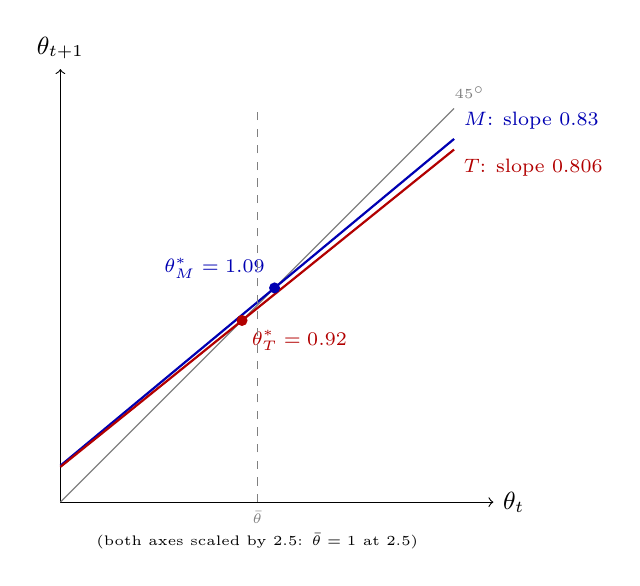
\begin{tikzpicture}[scale=1]
%% Phase diagram: theta_t+1 vs theta_t for both sectors
\draw[->] (0,0) -- (5.5,0) node[right, font=\small] {$\theta_t$};
\draw[->] (0,0) -- (0,5.5) node[above, font=\small] {$\theta_{t+1}$};
\draw[gray, thin] (0,0) -- (5,5); % 45-degree line
\node[font=\tiny, gray] at (5.2, 5.2) {$45^\circ$};

%% Modern sector: steeper, crosses higher
%% theta' = 0.83 theta + 0.185, drawn in coordinates scaled by 2.5 (code/ch09.py)
\draw[blue!70!black, thick] (0, 0.4625) -- (5, 4.6125);
\node[font=\scriptsize, blue!70!black, above right] at (5, 4.6125) {$M$: slope 0.83};

%% Traditional sector: flatter, crosses lower
%% theta' = 0.806 theta + 0.179, scaled by 2.5
\draw[red!70!black, thick] (0, 0.4475) -- (5, 4.4775);
\node[font=\scriptsize, red!70!black, below right] at (5, 4.4775) {$T$: slope 0.806};

%% Fixed points
\fill[blue!70!black] (2.72, 2.72) circle (2pt);
\node[font=\scriptsize, blue!70!black, above left] at (2.72, 2.72) {$\theta_M^* = 1.09$};
\fill[red!70!black] (2.307, 2.307) circle (2pt);
\node[font=\scriptsize, red!70!black, below right] at (2.307, 2.307) {$\theta_T^* = 0.92$};

%% Anchor line
\draw[dashed, gray] (2.5, 0) -- (2.5, 5);
\node[font=\tiny, gray, below] at (2.5, 0) {$\bar{\theta}$};

%% Scale note
\node[font=\tiny] at (2.5, -0.5) {(both axes scaled by 2.5: $\bar{\theta} = 1$ at 2.5)};
\end{tikzpicture}
\qquad
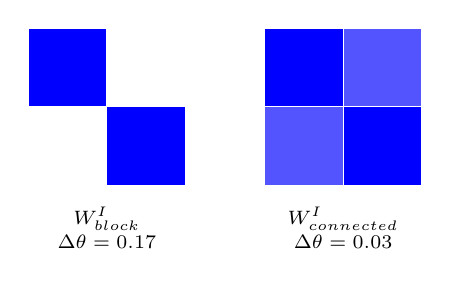
\begin{tikzpicture}[scale=1]
%% Two heatmaps showing W^I
\def\s{1.0}
%% Block-diagonal W^I
\foreach \i/\j/\v in {1/1/100,1/2/0,2/1/0,2/2/100} {
  \fill[blue!\v, draw=white, line width=0.3pt]
    ({(\j-1)*\s}, {(2-\i)*\s}) rectangle +(\s,\s);
}
\node[below, font=\scriptsize\bfseries] at ({\s}, -0.15) {$W^I_{\text{block}}$};
\node[below, font=\scriptsize] at ({\s}, -0.5) {$\Delta\theta = 0.17$};

\begin{scope}[xshift=3cm]
%% Connected W^I
%% weights 0.6/0.4 normalized to the matrix max
\foreach \i/\j/\v in {1/1/100,1/2/67,2/1/67,2/2/100} {
  \fill[blue!\v, draw=white, line width=0.3pt]
    ({(\j-1)*\s}, {(2-\i)*\s}) rectangle +(\s,\s);
}
\node[below, font=\scriptsize\bfseries] at ({\s}, -0.15) {$W^I_{\text{connected}}$};
\node[below, font=\scriptsize] at ({\s}, -0.5) {$\Delta\theta = 0.03$};
\end{scope}
\end{tikzpicture}
\end{center}
\vspace{-0.5em}
\small Left: phase diagram. Each map crosses the $45^\circ$ line once with slope below 1, so each agent has a unique stable steady state; the Modern agent's lies above the anchor $\bar{\theta}$ and the Traditional agent's below it. Right: with $W^I = I$ the preference gap is 0.17; a connected $W^I$ with weights $0.6/0.4$ reduces it to 0.03 (0.031). The gap comes from different returns, and $W^I$ decides how much of the other sector's returns each agent sees.
\end{vizpanel}


%% =====================================================================
\section{Persistence: Why the Past Lingers}
\label{ch09:sec:hysteresis}
%% =====================================================================

The formation equation has an important dynamic property: after $W^I$ changes, preferences adjust only gradually, and slowly if $\rho$ is close to 1.

\begin{proposition}[Persistence of Preferences]\label{ch09:thm:hysteresis}
Suppose $W^I$ changes from $W^I_{\text{old}}$ to $W^I_{\text{new}}$ at $t = 0$, starting from $\boldsymbol{\theta}_0 = \boldsymbol{\theta}^*_{\text{old}}$. Let $\boldsymbol{\theta}^*_{\text{new}}$ be a steady state of the new map, let $\mathbf{g}$ be differentiable there, and let
\begin{equation}\label{ch09:eq:local_rate}
J_{\text{new}} := \rho I + \mu W^I_{\text{new}}\, D\mathbf{g}(\boldsymbol{\theta}^*_{\text{new}}), \qquad \lambda := \rho(J_{\text{new}}) < 1.
\end{equation}
Then for every $\varepsilon > 0$ there are constants $C, \delta > 0$ such that, whenever $\|\boldsymbol{\theta}^*_{\text{old}} - \boldsymbol{\theta}^*_{\text{new}}\| < \delta$,
\begin{equation}\label{ch09:eq:hysteresis}
\|\boldsymbol{\theta}_t - \boldsymbol{\theta}^*_{\text{new}}\| \leq C \cdot (\lambda + \varepsilon)^t \cdot \|\boldsymbol{\theta}^*_{\text{old}} - \boldsymbol{\theta}^*_{\text{new}}\|.
\end{equation}
If $\mathbf{g}$ is affine the bound holds globally. The asymptotic half-life of preference adjustment is
\begin{equation}\label{ch09:eq:halflife}
t_{1/2} = \frac{\ln 2}{\ln(1/\lambda)} \quad \text{generations}.
\end{equation}
If returns are increasing in preferences ($D\mathbf{g} \geq 0$), then $\lambda \geq \rho$: complementarities slow adjustment down. $\lambda = \rho$ only when the formation signal does not respond to $\boldsymbol{\theta}$ ($D\mathbf{g} = 0$).
\end{proposition}

\begin{proof}
Write $T$ for the new map and $\Delta_t = \boldsymbol{\theta}_t - \boldsymbol{\theta}^*_{\text{new}}$. Since $T(\boldsymbol{\theta}^*_{\text{new}}) = \boldsymbol{\theta}^*_{\text{new}}$, we have $\Delta_{t+1} = J_{\text{new}}\Delta_t + o(\|\Delta_t\|)$. For any $\varepsilon > 0$ there is a vector norm $\|\cdot\|_\star$ whose induced matrix norm satisfies $\|J_{\text{new}}\|_\star \le \lambda + \varepsilon/2$ (a standard consequence of the Jordan form). Choose $\delta$ so that the remainder is at most $(\varepsilon/2)\|\Delta_t\|_\star$ on the $\delta$-ball. Then $\|\Delta_{t+1}\|_\star \le (\lambda+\varepsilon)\|\Delta_t\|_\star$; by induction the trajectory stays in the ball, and equivalence of norms gives the constant $C$. If $\mathbf{g}$ is affine, the remainder is zero. Finally, if $A := \mu W^I_{\text{new}}D\mathbf{g} \geq 0$, the eigenvalues of $J_{\text{new}} = \rho I + A$ are $\rho + \operatorname{eig}(A)$. By Perron--Frobenius $\rho(A)$ is itself an eigenvalue of $A$, so $\lambda = \rho + \rho(A) \geq \rho$.
\end{proof}

\begin{example}[Persistence Rates]\label{ch09:ex:hysteresis}
\textbf{Half-lives when the signal does not feed back ($\lambda = \rho$).} With $\rho = 0.9$, the half-life is $\ln 2 / \ln(10/9) \approx 6.6$ generations, or about 164 years at 25 years per generation.

Suppose, hypothetically, that a country's $W^I$ changed at $t = 0$ and $\lambda = 0.9$. One generation later 10\% of the gap to the new steady state has closed; after two generations 19\%; after four (a century) 34\%. Preferences formed under the old structure would still account for most of the gap a century later.

$\rho = 0.7$: half-life $= \ln 2 / \ln(10/7) \approx 1.9$ generations (49 years), about 3.4 times faster than $\rho = 0.9$.

$\rho = 0.5$: half-life $= 1$ generation (25 years).

\textbf{With feedback.} In Example~\ref{ch09:ex:two_steady}, the Modern agent's map has slope $\lambda = \rho + \mu g'_M = 0.8 + 0.3 \times 0.1 = 0.83$. The half-life is therefore $\ln 2/\ln(1/0.83) = 3.7$ generations, not the $3.1$ implied by $\rho = 0.8$ alone.

Which value of $\rho$ applies is an empirical question (Chapter~11). The table is a menu, not an estimate.

\begin{center}
\begin{tabular}{lccc}
\toprule
$\rho$ & $t_{1/2}$ (generations) & $t_{1/2}$ (years) & Speed \\
\midrule
0.95 & 13.5 & 338 & Glacial \\
0.90 & 6.6 & 164 & Slow \\
0.80 & 3.1 & 78 & Moderate \\
0.70 & 1.9 & 49 & Visible \\
0.50 & 1.0 & 25 & Fast \\
\bottomrule
\end{tabular}
\end{center}
\end{example}

\begin{keyinsight}
Persistence is one reason structural change can be slow. $W^P$ can change within a decade (a road, a factory), and $W^I$ within years (phones, a media campaign). But if $\lambda$ is close to 1, preferences formed under the \textit{old} $W^I$ persist for generations.

This means: (1) structural policies that change $W$ have a delayed effect on preferences --- the payoff is intergenerational, (2) evaluating policies using \textit{current} preferences underestimates their long-run impact, because current preferences were formed under the old structure, and (3) the welfare function itself changes over time --- which is the problem of Chapter~12.

Persistence can explain why countries with similar current institutions and prices have different outcomes: their preference vectors $\boldsymbol{\theta}$ reflect different histories of $W^I$. With a unique stable steady state this is slow convergence, not hysteresis. True path dependence --- where a temporary shock has permanent effects --- requires multiple steady states (Chapter~10).
\end{keyinsight}


%% =====================================================================
\section{Enforcement vs.\ Formation}
\label{ch09:sec:enforcement_formation}
%% =====================================================================

The standard model explains behavior through two channels: \textbf{prices} (you work more because wages rose) and \textbf{constraints} (you work more because the law changed). Both operate within a generation, holding $\boldsymbol{\theta}$ fixed. We call these \textbf{enforcement effects}: the structure enforces behavior through prices and constraints.

The formation model adds a third channel: \textbf{the structure changes $\boldsymbol{\theta}$}. You work more because your reference group works more, and observing them shifted your norm. This is the \textbf{formation effect}: the structure forms preferences.

\begin{definition}[Enforcement, Formation, and the $\Psi$ Ratio]\label{ch09:def:psi}
Fix an outcome $y_i = y_i(\boldsymbol{\theta}, W, \boldsymbol{\omega})$ for agent $i$: a behavior, an allocation, or a return. The economy starts at a steady state $\boldsymbol{\theta}^0 = \boldsymbol{\theta}^*(W)$. At $t = 0$ a permanent perturbation $\Delta W$ is applied. The perturbation must be stated explicitly: which layer ($W^P$, $W^I$, \ldots) changes, how its rows remain stochastic, or which transfer $\Delta\boldsymbol{\omega}$ is made. Let $\boldsymbol{\theta}_T$ be the preference vector $T$ generations later, generated by the formation equation under the new structure. Then:
\begin{align}
E_i(\Delta W) &:= y_i(\boldsymbol{\theta}^0, W + \Delta W) - y_i(\boldsymbol{\theta}^0, W), \label{ch09:eq:E}\\
F_i(\Delta W, T) &:= y_i(\boldsymbol{\theta}_T, W + \Delta W) - y_i(\boldsymbol{\theta}^0, W + \Delta W). \label{ch09:eq:F}
\end{align}
$E_i$ is the \textbf{enforcement effect} (the impact at fixed preferences); $F_i$ is the \textbf{formation effect} by horizon $T$.
The two effects add up to the total change, $E_i + F_i = y_i(\boldsymbol{\theta}_T, W+\Delta W) - y_i(\boldsymbol{\theta}^0, W)$. The \textbf{$\Psi$ ratio} of agent $i$ for perturbation $\Delta W$ at horizon $T$ is
\begin{equation}\label{ch09:eq:psi}
\Psi_i(\Delta W, T) := \frac{F_i(\Delta W, T)}{E_i(\Delta W)}, \qquad \text{defined when } E_i(\Delta W) \neq 0.
\end{equation}
The long-run ratio $\Psi_i(\Delta W, \infty)$ uses the new steady state, $\boldsymbol{\theta}_\infty = \boldsymbol{\theta}^*(W + \Delta W)$. The aggregate ratio is
\[
\bar{\Psi}(\Delta W, T) := \frac{\sum_i |F_i(\Delta W, T)|}{\sum_i |E_i(\Delta W)|}.
\] Absolute values are needed when allocations sum to a fixed total, because then $\sum_i E_i = \sum_i F_i = 0$.
\end{definition}

This is the only definition of $\Psi$ used in the book. Chapter~10 computes it inside the formation model. Chapter~11 discusses statistics that are related to it but are not the same object.

\begin{remark}[Reading $\Psi$]\label{ch09:rem:psi}
\begin{enumerate}
\item $\Psi$ is a property of a \textit{perturbation, an outcome, an agent, and a horizon}, not of an economy. The same economy has different $\Psi$ for a transfer and for a road.
\item $\Psi_i(\Delta W, 0) = 0$, and if $\mu = 0$ then $F_i \equiv 0$ for every perturbation: with exogenous preferences (A6) the benchmark model is complete.
\item $\Psi > 0$: formation reinforces enforcement. $\Psi > 1$: most of the change by horizon $T$ comes from preference change. $\Psi < 0$: formation offsets enforcement. That is possible; nothing forces the two effects to share a sign.
\item An evaluation that ignores formation captures the share $1/(1+\Psi)$ of the total effect at horizon $T$ and misses the share $\Psi/(1+\Psi)$ (for $\Psi > -1$).
\item When $E_i = 0$, $\Psi_i$ is undefined. This happens, for example, for a pure information policy whose outcome does not depend on $W^I$ at fixed preferences. Report $F_i$ itself in that case.
\end{enumerate}
\end{remark}

Chapter~11 asks what data can reveal about $\Psi$. The short answer: less than one would like, and only under strong assumptions.


%% =====================================================================
\section{The Self-Confirming Trap}
\label{ch09:sec:trap}
%% =====================================================================

\begin{proposition}[Block-wise Steady States]\label{ch09:thm:self_confirming}
Suppose the hypotheses of Proposition~\ref{ch09:prop:steady} hold, $W^I$ is block-diagonal with blocks $B_1, \ldots, B_k$, uniform weights within blocks, and identical return functions within each block that depend only on the block's own preferences. Then a steady state exists in which every agent of block $b$ has the same preference $\theta^*_b$, satisfying
\begin{equation}\label{ch09:eq:self_confirming}
\theta^*_b = \bar{\theta} + \frac{\mu}{1-\rho}\left(\bar{r}_b(\theta^*_b) - r^*\right),
\end{equation}
where $\bar{r}_b(\theta^*_b)$ is the average return within block $b$ at steady state. Each block's preference level is \textit{consistent with the returns it observes}: agents in block $b$ observe $\bar{r}_b$ and form the $\theta^*_b$ that those returns sustain.
\end{proposition}

\begin{proof}
With block-diagonal $W^I$, the formation equation decomposes: agents in block $b$ observe only returns from block $b$, and with uniform within-block weights every agent of the block receives the same signal $\bar{r}_b - r^*$. Apply Proposition~\ref{ch09:prop:steady} to the block's restricted map. Its fixed points include block-symmetric ones: restrict the map to the (compact, convex, or affine) set of block-constant vectors, which it leaves invariant.
\end{proof}

\begin{intuition}[The deepest trap]
The block-wise steady state is one way to formalize the idea behind the phrase ``culture of poverty'' --- without its pejorative connotation, and with the cause placed in the structure rather than in the people.

In the model, an agent in the traditional sector is not ``poor because she has low aspirations.'' She has low aspirations because $W^I$ shows her only traditional-sector returns. If she observed the modern sector's returns, she would form higher aspirations. Whether that helps her depends on whether those returns are \textit{attainable} for her. In Example~\ref{ch09:ex:two_steady} her own return function is $g_T$, and an aspiration calibrated on $g_M$ would overshoot what her sector rewards. The Prebisch box below is a case where the imported signal does harm. An edge in $W^I$ is not good or bad in itself; what matters is whether the returns it carries are relevant to the observer.

So part of the problem lies in the network, not in the preferences. Change $W^I$ \textit{together with} access to the observed returns (the scholarship, the job network, the mentor in the modern sector), and the preferences change. Leave $W^I$ and the return structure unchanged, and the preferences persist.

This is Furtado's ``autonomous process of underdevelopment'' (Chapter~2) applied to preferences: the structure produces the preferences that justify the structure.
\end{intuition}

\begin{prebisch}[Demonstration effect and cultural dependency]
\citet{nurkse1953problems} called it the international ``demonstration effect'', extending \citeauthor{duesenberry1949income}'s (\citeyear{duesenberry1949income}) idea: consumers in poorer countries emulate the consumption standards of richer ones, which depresses saving. \citet{furtado1974mito} made it a pillar of cultural dependency. Income concentration lets a peripheral minority reproduce centre consumption patterns, and that composition of demand then shapes what the periphery's industry produces and which techniques it imports. Prebisch's late work \citep{prebisch1981capitalismo} attacked the same ``privileged consumer society''.
% TODO-VERIFY: Prebisch (1981) "sociedad privilegiada de consumo" wording and page in Capitalismo periferico.
In network terms, peripheral elites observe centre lifestyles through $W^I$ (travel, media, education abroad) and form consumption preferences calibrated to centre income levels.

In the formation equation: the peripheral elite's $W^I$ has cross-border edges to the center. They observe $r_{\text{center}}$ (high consumption, high variety) and form $\theta^*_{\text{elite}}$ calibrated to those signals. But their income is peripheral, so the gap between aspirations and means is large. They consume rather than save. The modern-sector investment that would close the gap does not occur.

This is the mirror image of the traditional-sector case above. There, \textit{too few} cross-block edges kept aspirations low; here, cross-border edges carry signals that are \textit{not attainable} at peripheral incomes. The elite's preferences are consistent with what it observes, but the consequences are self-defeating: too little is invested. The formation equation by itself cannot say whether an edge helps or harms. That depends on whether the observed returns are attainable by the observer --- a point that returns in Chapter~12.
\end{prebisch}


%% =====================================================================
\section{Summary}
\label{ch09:sec:summary}
%% =====================================================================

\begin{enumerate}
\item \textbf{Five preference parameters} that the benchmark model treats as exogenous --- time discount, aspiration level, labor supply, risk tolerance, taste for variety --- vary systematically with the social and informational environment. Much of this evidence concerns beliefs and norms rather than tastes, so Part~III treats $\theta$ as a reduced-form behavioral parameter.

\item The \textbf{formation equation} $\theta_{i,t+1} = \rho\theta_{i,t} + (1-\rho)\bar{\theta} + \mu(\sum_j W^I_{ij} r_{j,t} - r^*)$, with $t$ indexing generations of a dynasty, has three components: intergenerational persistence ($\rho$), anchor ($\bar{\theta}$), and network signal. Steady states exist under stated conditions (bounded returns, or affine returns with a nonsingular system). Heterogeneous returns produce heterogeneous steady states; that is not multiplicity.

\item \textbf{Persistence}: after $W^I$ changes, preferences converge at the local rate $\lambda = \rho(\rho I + \mu W^I D\mathbf{g})$, which is at least $\rho$ when returns rise with preferences. The half-life is $\ln 2/\ln(1/\lambda)$ generations: 6.6 generations (about 164 years) if $\lambda = 0.9$.

\item The \textbf{$\Psi$ ratio} $\Psi_i(\Delta W, T) = F_i/E_i$ compares formation and enforcement effects for a stated perturbation, outcome and horizon. It is not a property of the economy, and it can be negative or undefined.

\item \textbf{Block-wise steady states}: with block-diagonal $W^I$, each block forms preferences consistent with the returns it observes. Whether adding an edge helps depends on whether the returns it carries are attainable by the observer --- the traditional-sector case and Furtado's demonstration effect point in opposite directions.
\end{enumerate}


%% =====================================================================
\section{Exercises}
\label{ch09:sec:exercises}
%% =====================================================================

\begin{enumerate}[label=\textbf{9.\arabic*}, leftmargin=3em]

\item \textbf{The formation equation by hand.} For $\rho = 0.8$, $\bar{\theta} = 1$, $\mu = 0.2$, $r^* = 0.1$, and a constant return $r = 0.15$:
\begin{enumerate}
\item Starting from $\theta_0 = 0.5$, compute $\theta_1, \theta_2, \ldots, \theta_{10}$ by hand.
\item Compute the steady state $\theta^*$ analytically. Verify convergence.
\item Plot the trajectory. How many periods to reach 90\% of the steady state?
\item Now set $\rho = 0.95$ and repeat. How does the convergence speed change?
\end{enumerate}

\item \textbf{Heterogeneous steady states.} Reproduce Example~\ref{ch09:ex:two_steady}:
\begin{enumerate}
\item Verify the steady-state values $\theta_M^* = 1.088$ and $\theta_T^* = 0.923$.
\item Now connect the blocks: $W^I = \begin{pmatrix} 0.7 & 0.3 \\ 0.3 & 0.7 \end{pmatrix}$. Compute the new steady states.
\item How large must the cross-block weight be for the two steady-state preferences to coincide? Why does the gap vanish exactly there?
\item Interpret: what real-world intervention corresponds to increasing $W^I_{12}$?
\end{enumerate}

\item \textbf{Persistence in female labor supply.} Suppose the norm for female market labor is $\theta^F$ (the share of time allocated to market work). The formation equation: $\theta^F_{t+1} = 0.85\theta^F_t + 0.15 \times 0.5 + 0.1(\bar{r}_t - 0.1)$, where $\bar{r}_t = 0.3\theta^F_t$ (returns are proportional to participation rate --- network effects in labor markets).
\begin{enumerate}
\item Compute the steady state. Is it unique?
\item Starting from $\theta^F_0 = 0.2$ (low participation): simulate 50 generations. Plot the trajectory.
\item At generation 10, WWII occurs: $\theta^F_{10}$ jumps to 0.6 (women enter factories). Simulate the post-war trajectory. Does $\theta^F$ return to the pre-war level?
\item In this linear model the steady state is unique, so the war has \textit{no} permanent effect. Show this. What feature would the model need for a temporary shock to have a permanent effect? (Hint: an S-shaped return function, Chapter~10.) Compare the empirical evidence on WWII mobilization and later female participation (e.g.\ \citealp[\textit{QJE}, ``Mothers and Sons'']{fernandez2004mothers}).
\end{enumerate}

\item \textbf{Aspiration and the smartphone.} Use the parameters and return functions of Example~\ref{ch09:ex:two_steady}. An agent in the traditional sector has $\theta^T_0 = 0.8$ (low aspiration). At $t = 5$, she gets a smartphone that adds a cross-block edge in $W^I$: she now observes modern-sector returns with weight 0.3.
\begin{enumerate}
\item Compute the old steady state (block-diagonal $W^I$) and the new steady state (with the cross-block edge).
\item Simulate the transition. How many generations to close half the aspiration gap?
\item What if 100 agents get smartphones simultaneously? Does the aggregate effect equal 100 times the individual effect? (Hint: the returns function may change when many agents shift behavior.)
\end{enumerate}

\item \textbf{\citet{bernard2014future} as a $W^I$ perturbation.} In the Ethiopian aspiration experiment:
\begin{enumerate}
\item Model the documentary as adding edges in $W^I$ from ``successful farmer'' (the film subject) to the treated farmers. Write the perturbation $\Delta W^I$.
\item Compute the change in steady-state aspirations $\Delta\theta^*$ as a function of $\mu$, $\rho$, and the film subject's return $r_{\text{film}}$.
\item Suppose the documentary raised aspirations by 0.1 SD at six months (an illustrative figure). What would this imply about $\mu$? What is the problem with mapping a six-month effect into a per-generation parameter?
\item The effect on savings was larger than the effect on aspirations. Can the formation model explain this? (Hint: savings = $f(\theta)$ may be convex.)
\end{enumerate}

\item \textbf{The $\Psi$ ratio for education.} Use Definition~\ref{ch09:def:psi} with outcome $x$ and horizon $T = 1$. In a simple model where $x = \theta \cdot w / p$ (quantity demanded is proportional to $\theta$ times real income):
\begin{enumerate}
\item A policy cuts the price of education by 10\% (enforcement). Compute $\Delta x / x$.
\item The same policy, by increasing returns to educated women in the girl's reference group, raises $\theta$ by 5\% over one generation (formation). Compute the additional $\Delta x / x$.
\item What is $\Psi$? Which effect is larger?
\item Under what conditions does the formation effect exceed the enforcement effect ($\Psi > 1$)?
\end{enumerate}

\item \textbf{Furtado's demonstration effect.} In a two-country model (Center, Periphery):
\begin{enumerate}
\item The Peripheral elite observes the Center's consumption through $W^I$ (travel, media). Model this as $W^I_{\text{elite, Center}} = 0.4$, $W^I_{\text{elite, Periphery}} = 0.6$.
\item The Center's consumption-to-income ratio is 0.85 (high consumption). The Periphery's sustainable ratio is 0.70 (lower income, needs more saving). Let $\theta$ be the elite's consumption-to-income ratio, with formation equation~\eqref{ch09:eq:formation}, anchor $\bar{\theta} = 0.70$, reference $r^* = 0.70$, $\rho = 0.9$ and $\mu = 0.4$ (so $\mu/(1-\rho) = 4$). The observed ``returns'' are the two consumption ratios. Compute the elite's steady-state $\theta^*$.
\item At what $W^I_{\text{elite, Center}}$ does the elite's steady-state consumption-to-income ratio exceed 1 (chronic dissaving)?
\item This is Furtado's ``myth of development'': the periphery consumes as if it were the center. What structural change would break the pattern?
\end{enumerate}
\end{enumerate}


%% =====================================================================
\newpage
\section*{Mathematical Appendices}
\addcontentsline{toc}{section}{Mathematical Appendices}
%% =====================================================================


\subsection*{Appendix 9A: Fixed Points of the Formation Mapping}
\addcontentsline{toc}{subsection}{Appendix 9A: Fixed Points of the Formation Mapping}
\label{ch09:app:fixed}

\paragraph{The formation mapping.} Define $\Phi: \R^N \to \R^N$ by:
\begin{equation}
\Phi_i(\boldsymbol{\theta}) = \bar{\theta} + \frac{\mu}{1-\rho}\left(\sum_j W^I_{ij} g_j(\boldsymbol{\theta}) - r^*\right).
\end{equation}
The steady state $\boldsymbol{\theta}^*$ is a fixed point: $\Phi(\boldsymbol{\theta}^*) = \boldsymbol{\theta}^*$.

\paragraph{Existence.} If each $g_j$ is continuous and bounded by $B$, then $\Phi$ maps the compact convex cube $\Theta = \{\|\boldsymbol{\theta} - \bar{\theta}\ones\|_\infty \le \frac{\mu}{1-\rho}(B + |r^*|)\}$ into itself, and Brouwer's theorem gives a fixed point. With unbounded (e.g.\ affine) $g$, Brouwer does not apply directly. In the affine case $\mathbf{g} = \mathbf{a} + G\boldsymbol{\theta}$, the fixed-point condition is linear, and a unique fixed point exists iff $I - \frac{\mu}{1-\rho}W^IG$ is nonsingular.

\paragraph{Uniqueness.} $\Phi$ has a unique fixed point if it is a contraction: $\|\Phi(\boldsymbol{\theta}) - \Phi(\boldsymbol{\theta}')\|_\infty \leq q\|\boldsymbol{\theta} - \boldsymbol{\theta}'\|_\infty$ for some $q < 1$ on the whole domain (Banach). When $g_j$ depends only on $\theta_j$, a valid constant is $q = \frac{\mu}{1-\rho}\|W^I\|_\infty \cdot \max_j \sup_\theta |g'_j(\theta)|$, with $\|W^I\|_\infty = 1$ for row-stochastic $W^I$. Uniqueness is guaranteed when $\frac{\mu}{1-\rho}\max_j\sup|g'_j| < 1$. This condition is sufficient, not necessary.

\paragraph{Multiple equilibria.} When $\frac{\mu}{1-\rho}$ is large and $g_j$ has a steep enough segment (an S-shape), the contraction condition fails and multiple steady states \textit{can} exist; Chapter~10 (Example~\ref{ch10:ex:trap}) gives one with three. Example~\ref{ch09:ex:two_steady} is \textit{not} such a case: there $q = 1.5 \times 0.1 = 0.15 < 1$, so each agent has a unique steady state, and the two values differ only because the return functions differ.


\subsection*{Appendix 9B: The Timescale Separation}
\addcontentsline{toc}{subsection}{Appendix 9B: Timescale Separation}
\label{ch09:app:timescale}

\paragraph{The two-timescale system.} The combined system is:
\begin{align}
\text{Fast:} \quad & \x_t = \x^*(\boldsymbol{\theta}_t, W) \quad \text{(within-period equilibrium)} \\
\text{Slow:} \quad & \boldsymbol{\theta}_{t+1} = \rho\boldsymbol{\theta}_t + (1-\rho)\bar{\theta}\ones + \mu(W^I \mathbf{g}(\x_t) - r^*\ones) \quad \text{(formation)}
\end{align}

\paragraph{Slow--fast scaling.} A clean slow--fast analysis separates the \textit{speed} of preference adjustment from the \textit{long-run sensitivity} to the signal. Write $\varepsilon := 1 - \rho$ and $\mu = \varepsilon\kappa$, so that
\[
\boldsymbol{\theta}_{t+1} - \boldsymbol{\theta}_t = \varepsilon\left[(\bar{\theta}\ones - \boldsymbol{\theta}_t) + \kappa\,(W^I\mathbf{g}(\x_t) - r^*\ones)\right].
\]
The steady state depends on $\kappa = \mu/(1-\rho)$ but not on $\varepsilon$, and $\varepsilon$ alone sets the speed. In the limit $\varepsilon \to 0$ with $\kappa$ fixed, preferences are frozen on any finite horizon and only enforcement effects operate. Over $t \sim 1/\varepsilon$ generations they follow the ODE $\dot{\boldsymbol{\theta}} = \bar{\theta}\ones - \boldsymbol{\theta} + \kappa(W^I\mathbf{g} - r^*\ones)$. Letting $\rho \to 1$ with $\mu$ fixed instead would send the steady-state deviation $\mu/(1-\rho)$ to infinity --- one reason to report $\kappa = \mathcal{M}$ (Chapter~10) and $\varepsilon$ separately.

\paragraph{Identification.} The idea behind Chapter~11's two-step strategy: the fast dynamics would identify demand and supply parameters at fixed $\boldsymbol{\theta}$, and the slow dynamics would identify $(\rho, \mu, \bar{\theta})$ from across-cohort variation. Chapter~11 shows what this requires: a restriction on age, period and cohort effects; a way to deal with the reflection problem; and a measured $W^I$.


%% =====================================================================
\subsection*{Structuralist Case Study: Furtado's \textit{O Mito do Desenvolvimento} and Cultural Dependency}
\addcontentsline{toc}{subsection}{Structuralist Case Study: Furtado (1974)}
%% =====================================================================

In 1974, while in exile and teaching in Paris, Celso Furtado published \textit{O Mito do Desenvolvimento Econ\^{o}mico} \citep{furtado1974mito}, a short book that pushed his analysis of underdevelopment into the domain of \textbf{culture, consumption patterns, and the social construction of desire}.

Furtado's earlier work (\textit{Desenvolvimento e Subdesenvolvimento}, \citeyear{furtado1961desenvolvimento}) had analyzed the production structure --- in this book's terms, the block-diagonal $W^P$. As the first head of SUDENE (from 1959) he had tried to change that structure through policy. \textit{O Mito} asked a different question: \textit{even if you change $W^P$, will it matter if the preferences of peripheral agents are calibrated to the center?}

The argument has three parts.

\textbf{Part 1: The myth of development is the belief that peripheral countries can replicate center consumption patterns.} Furtado argued that ``development'' as understood in the postwar period meant achieving center-level consumption: automobiles, appliances, industrialized food, suburban housing. This consumption pattern was not a natural aspiration but a \textit{culturally constructed} one, transmitted to the periphery through $W^I$ (advertising, education, media, elite travel). In the formation equation~\eqref{ch09:eq:formation}: the return $r_{j,t}$ observed by the peripheral elite is center-level consumption, filtered through $W^I$ edges that connect peripheral elites to center lifestyles. The formation signal pushes $\theta_i$ (taste for consumption) upward, toward the center's steady state.

\textbf{Part 2: Center consumption patterns at peripheral income levels produce structural distortion.} If $\theta_i$ (consumption aspiration) is calibrated to center returns but income is peripheral, the savings rate collapses: agents consume beyond their means, relying on debt, capital inflows, or natural resource rents. For Furtado the mechanism is distributive and structural. Income concentration allows a minority to reproduce centre consumption patterns. That composition of demand then directs industrialization toward goods and techniques designed for centre incomes, while the majority is excluded from the modern consumption pattern rather than merely ``unambitious''. In the model, block-wise steady states (Section~\ref{ch09:sec:trap}) operate through the consumption channel: the elite's $\theta_{\text{consumption}}$ is centre-calibrated, saving and broad-based investment are low, and $W^P$ stays block-diagonal. Furtado's emphasis on exclusion is a statement about \textit{access} (who can attain which returns), which the formation equation alone does not represent.

\textbf{Part 3: The ecological impossibility.} Furtado's most prescient argument: even if every country could replicate center consumption, the planet cannot sustain it. The myth of development is a myth not only because the periphery cannot achieve it within the existing power structure, but because \textit{nobody} can achieve it within the planet's ecological constraints. This was 1974, two years after \textit{The Limits to Growth} \citep{meadows1972limits}, which Furtado discusses explicitly. In the formation framework: the centre's $\boldsymbol{\theta}^*$ is not a feasible global steady state. It is a local configuration sustained by the centre's disproportionate claim on global resources (Chapter~16). This part of the argument is not formalized in this chapter.

\begin{center}
\begin{tabularx}{\textwidth}{LLL}
\toprule
\textbf{Furtado's argument (1974)} & \textbf{Formal object} & \textbf{This chapter} \\
\midrule
Consumption aspirations are culturally formed & $\theta_{i,t+1} = f(W^I, r_{j,t})$ & Def.~\ref{ch09:def:formation} \\
Peripheral elites observe center lifestyles & $W^I_{\text{elite, center}} > 0$ & Sec.~\ref{ch09:sec:formation} \\
High aspiration at low income = undersaving & $\theta_{\text{cons}}$ high, $Y$ low $\to$ $S$ low & Prebisch box \\
Underdevelopment reproduces itself culturally & Block-wise steady states & Prop.~\ref{ch09:thm:self_confirming} \\
Past structures persist in current preferences & Persistence at rate $\lambda \geq \rho$ & Prop.~\ref{ch09:thm:hysteresis} \\
The myth is a myth for everyone & Center $\boldsymbol{\theta}^*$ not globally feasible & Not formalized here (Ch.~16, Ch.~26) \\
\bottomrule
\end{tabularx}
\end{center}

\textit{O Mito} was Furtado at his most radical. He had started in 1961 by saying underdevelopment was a structural condition of $W^P$. By 1974 he was also saying that underdevelopment is reproduced through consumption patterns and culture --- in this book's terms, through $\boldsymbol{\theta}$ as well as $W^P$. The production structure helps produce the preferences that sustain it. On this reading, changing $W^P$ is necessary but not sufficient: $W^I$ --- the channel through which the structure becomes desire --- and access to the returns it displays must change too.

He did not have the formation equation. He had the argument: that the most insidious form of dependence is not economic but \textit{cultural} --- the colonization of what you want. This chapter gives that argument its dynamics.


%% =====================================================================
\subsection*{Further Reading}
\addcontentsline{toc}{subsection}{Further Reading}
%% =====================================================================

\textbf{Endogenous preferences:} \citet{bowles1998endogenous}, ``Endogenous Preferences: The Cultural Consequences of Markets and Other Economic Institutions.'' \citet{bisin2001economics}, ``The Economics of Cultural Transmission and the Dynamics of Preferences.'' \citet{bisin2011economics}, ``The Economics of Cultural Transmission and Socialization,'' in Benhabib, Bisin, and Jackson (eds.), \textit{Handbook of Social Economics}.

\textbf{Aspirations:} \citet{ray2006aspirations}, ``Aspirations, Poverty, and Economic Change,'' in Banerjee, B\'{e}nabou, and Mookherjee (eds.), \textit{Understanding Poverty}. \citet{bernard2014future}, ``The Future in Mind: Aspirations and Forward-Looking Behaviour in Rural Ethiopia,'' CSAE WP. \citet{genicot2017aspirations}, ``Aspirations and Inequality.''

\textbf{Cultural transmission and labor:} \citet{fernandez2013cultural}, ``Cultural Change as Learning: The Evolution of Female Labor Force Participation over a Century.'' \citet{fernandez2007women}, ``Women, Work, and Culture.'' \citet{fernandez2004mothers}, ``Mothers and Sons.'' \citet{fogli2011nature}, ``Nature or Nurture? Learning and the Geography of Female Labor Force Participation.'' \citet{fernandez2009culture}, ``Culture: An Empirical Investigation.''

\textbf{Risk and experience:} \citet{malmendier2011depression}, ``Depression Babies: Do Macroeconomic Experiences Affect Risk Taking?''

\textbf{The structuralist tradition on culture:} \citet{furtado1974mito}, \textit{O Mito do Desenvolvimento Econ\^{o}mico}, Rio de Janeiro: Paz e Terra (the primary source). \citet{furtado1978criatividade}, \textit{Criatividade e Depend\^{e}ncia na Civiliza\c{c}\~{a}o Industrial}, also from exile. \citet{nurkse1953problems}, \textit{Problems of Capital Formation in Underdeveloped Countries} (the international demonstration effect). \citet{prebisch1981capitalismo}, \textit{Capitalismo Perif\'{e}rico}.

\textbf{Beliefs versus tastes; social capital:} \citet{becker1996accounting}, \textit{Accounting for Tastes}. \citet{becker2000social}, \textit{Social Economics}. \citet{bursztyn2014understanding}, ``Understanding Mechanisms Underlying Peer Effects.'' \citet{dietrich2013where}, ``Where Do Preferences Come From?''

\end{document}
